% Text:              √
% Citations:         X
% Revision:          X
% Final Revision:    X
\chapter{Preliminaries}
This chapter aims to provide a context for the thesis.
The reader will be able to gain the necessary background knowledge in order
to understand the purpose of the thesis and why it can be useful for developing Jolie applications. This 
essentially builds on the motivation
described in the previous chapter.

This chapter will highlight some of the relevant definitions and concepts of the microservice architecture paradigm, some of the benefits and consequences, as
 well as provide
the reader with a quick overview of the Jolie programming language,
what Docker Compose is, and what tools exist both for Jolie and
other programming languages which can be used in some way to visualize.

\section{Microservice Architecture}
Building software requires a lot of careful considerations when it comes
to choosing a software architecture. Many developers will choose a more monolithic architecture where all
 the functionality of the application
is in one codebase. This seems like the simpler approach because everything is deployed as one solution, however,
 there are many drawbacks
with this approach when the software starts getting bigger, and a larger number of users starts
interacting with the platform.

For this section and the following subsections, the book \textit{Microservices Patterns} by Chris Richardson \cite*{microservicepatterns} will serve as a good foundation. 
The definitions and concepts described by him will be used throughout this thesis.

\subsection{Some of the Problems with Monoliths}
Drawbacks exist in all parts of using monolith software architecture, everything from development to
deploying and maintaining the production application.
From a development standpoint, it can be slow to introduce new features into a monolithic application's
 codebase. As the project grows, so will the complexity, and trying to somehow weave in a new feature in a large, cluttered project can seem almost impossible.

After developing a new feature, or fixing a bug, the developer would ideally like to see their change
in production as fast as possible. This can, however, be a long and tedious process when developing in one large codebase.
First, all tests must run, which can take a long time. The codebase is complex so the likelihood of a
test failing is big, meaning that the tests must be run multiple times.

When the project runs in production, a whole new set of issues can quickly arise. It can be difficult
to scale an application when the whole application is one big instance.
The only thing to do is give the machine running the application more processing power and memory
storage capacity, in other words, vertically scale the application. Another significant problem with having the application be one instance of everything, is that a single point of failure exists. If one functionality of the program is faulty, it can affect other parts of the application
even if the other parts seemingly have nothing to do with the faulty code.

\subsection{Utilizing the Microservice Architecture}
To avoid all the problems with the monolith architecture, developers can try to go for a more
 distributed approach, where the microservice architecture is one of those approaches.

The microservice architecture aims to make the application modular. This means that all business logic is broken up into different services 
where each service serves only one cohesive set of purposes, and the services can be replicated.
The services will have some API which other services can use for communication. This provides some forced boundary because a service can never access the internal classes and code of another service unless the API allows it.
This helps in preserving modularity and keeps services decoupled.
The definition of a microservice can be a bit indistinct, so it is often up to the individual development team what a microservice entails.

The microservice architecture also addresses the more \textit{non-functional} aspects of the application.
This includes maintainability, extensibility and testability, as well as the important aspect of
\textit{horizontal scaling} where multiple instances of the same business logic can be deployed giving 
faster response times and eliminating the single point of failure mentioned before.

There can be some difficulties in working with microservices, so it is not a one-solution-fits-all.
The communication between microservices can be a whole new dimension of complexity. The developer has several ways of implementing communication
and all have their benefits and consequences. The microservices can communicate through event channels, they can expose a REST API, and one could set up a service mesh to handle inter-service communication.
Another set of problems is data consistency. Different patterns can be used to ensure that data between services stay consistent. This includes \textit{sagas}, \textit{event sourcing} and many more.
% TODO write something more here

\section{Microservice API Patterns}
This section aims to highlight some microservice API patterns which have been discussed in the book by Olaf Zimmermann et al.

As mentioned before, microservices often communicate with each other through defined APIs and often the client of a microservice application will also communicate using an API.
Thinking about and incorporating good design patterns when creating any service-oriented architecture can be a big benefit.
The design patterns can be partitioned into five categories of design patterns each trying to solve different problems.

The first category of patterns is the \textit{Foundation Patterns}. These patterns aim to deal with executive decisions of the APIs, including: Where the API should be
accessible from, how a client interacts with the system through an API and how is the system landscape with multiple services handled. Some of the patterns in this category include frontend- and backend integration which aims
to address the communication between the client and the system and the communication between systems or services, respectively. Another set of patterns in this category is concerning the visibility of an API.

The second category is the \textit{Responsibility Patterns}, which aims to clarify the architectural roles and responsibilities of API endpoints.
This can be further partitioned into operational responsibilities, which aim to handle state changes from the API client, and information holder types which aim to handle the exchange of data between APIs and clients.

Diving deeper down the levels of abstraction, the third category, \textit{Structure Patterns}, addresses the structure of messages between APIs. This includes request parameters and responses.

The last category, which will be quickly explained in this part of the section, is the \textit{Evolution Patterns} which will address how the APIs evolve and how the API provider will handle versioning, compatibility and deprecation.

\subsection{Quality Patterns}
This category of patterns is highlighted in a subsection because they are more relevant in the context of the thesis. 
Quality patterns focus on cost-effectively providing high-quality services. These patterns can be partitioned into \textit{Refecence Management}, \textit{Data Transfer Parsimony}, and \textit{Quality Management and Governance}.

Relevant patterns in this category include the \textit{Conditional Request} pattern which aims to eliminate unnecessary server-side 
processing, the \textit{Rate Limit} pattern that prevents excessive usage of an endpoint and the \textit{Pricing Plan} pattern that allows the provider to monetize the API,

Many of the patterns can be used in conjunction to enhance the effect of the desired functionality. For example: \textit{Pricing Plan} can use \textit{Rate Limit} to allow the provider to have different levels of pricing plans.
To further enhance the functionality of the pricing plan pattern, \textit{API Keys} (A structure API pattern which allows the API provider
to assign a unique token/key to each client which can be used for authorization purposes) can be used together to allow the API provider to safely and reliably monetize the API using different billing plans. 
Adding this to an API Gateway is good to ensure that all clients are monetized accordingly.

Generally, most of the API patterns described in the book are best utilized in conjunction,
and when looking at Jolie in a moment, it is crucial to understand that these patterns, both API and non-API patterns,
should be seen as building blocks which are used together to implement the desired architecture.
It is also worth mentioning that the patterns discussed in this section will not be implemented in this thesis.


\section{Jolie}
Jolie is a service-oriented programming language, where (micro)services are the basic building blocks.
Everything in Jolie is contained in services and services communicate with each other through APIs which the programmer needs to design and implement in the code. \cite{jolie}

\subsection{Basic Building Blocks of a Jolie Program}
This subsection will quickly describe some of the relevant building blocks which are needed for a Jolie service.

\textbf{Service}: the service block is sort of the key element of Jolie programs. Everything inside this block is what that specific service will handle. It is also 
in this block where a developer will create business logic and provide information about the API. Services usually consist of some main business logic block and any number of ports.

\textbf{Ports}: ports are the means of communication between services. Not just between Jolie services but also external communication.
Jolie-services differentiate between in-going and out-going communication. So building blocks for both exists, namely \texttt{inputPort} and \texttt{outputPort}.
Ports have their properties which a developer needs to specify. The three main properties of any port are: \textit{location}, \textit{protocol}, and \textit{interfaces}.
Where location specifies where the port will be listening for messages and where the port will send messages.
The protocol specifies how the port sends and receives messages. Lastly, for input ports, interfaces specify which
operations the service is capable of performing, and for output ports, the interfaces specify which
operations the service is capable of invoking internally. Listing \ref*{lst:simple-inputport} shows a basic input port in Jolie, where all the key properties are set.

\begin{jolisting}[][caption={Simple input port in Jolie},label=lst:simple-inputport]
inputPort IP {
    Location: "socket://localhost:9999"
    Protocol: sodep
    Interfaces: SomeInterface
}
\end{jolisting}

The location of the port can utilize different media for communication, but the two most common are TCP/IP sockets and Jolie in-memory communication.
Specifying the location of ports with \texttt{socket://} followed by an IP address means that the ports are communicating via TCP/IP.
Specifying the location with \texttt{local} means that the ports will use an in-memory channel to communicate, this also means that services on different networks cannot communicate.
A port using the local communication medium will be referred to as a "local port".

\textbf{Interfaces}: interfaces define a list of operations, which a service needs to implement in order to use. These operations can be of type \texttt{RequestResponse}, where the operation takes in some request type and return some response type, 
and \texttt{OneWay} where the operation takes in a request type but returns nothing. The syntax of a RequestResponse operation is: \jo{opName(RequestType)(ResponseType)}, and for OneWay operations it is: \jo{opName(RequestType)}

\textbf{Type}: interfaces use types to define what is expected to be given to an operation, and in some cases what the operation will return. In Jolie, there are basic
data types which include: \texttt{void}, \texttt{int}, \texttt{string}, \texttt{bool}, etc. However, it is also to define custom types which can contain subtypes.
This could be used when an operation needs more data types.
Listing \ref*{lst:type-with-interf} is an example of a custom type used in an interface in Jolie:
\begin{jolisting}[][caption={Custom type used in an interface in Jolie},label=lst:type-with-interf]
type SomeType: void {
    content: string
    id: int
}

interface SomeInterface {
    RequestResponse:
        someOperation(SomeType)(int)
}
\end{jolisting}

Besides the four things mentioned, there are some other things which are needed for a Jolie program, however, for this thesis, there is no reason to dive further into the specifics.
If one wishes to get more familiar with the language, the programming language does have a documentation page which goes more into the specifics of each component.

\subsection{Embedding Services in Jolie}
Jolie facilitates the possibility of programming the execution contexts.
This means that, in code, the developer can handle the execution of other services. This is called \textit{Embedding}.

A service can embed another service, which means that the embedder can launch the embedded service. This is useful when a service depends on another service to be running.
The service can simply embed another service to ensure that when the embedder is running, so is the embedded services.
Another benefit of embedding is that the language will take care of the connection, meaning that the developer does not necessarily need to worry about how a service is connected to the embedded services.
This also potentially hides the connection from the outside world.

The in-memory communication channel can be utilized here. The developer can specify if the embedder should create a new local port and connect automatically via that. This requires that the embedded service contains an input port which shares protocol and location.
Listing \ref*{lst:embed-as} showcases this functionality.

\begin{jolisting}[][caption={Embedding of a service called "svc" via a local output port "OP"}, label=lst:embed-as]
embed svc as OP
\end{jolisting}

It is not required that the embedder specifies some local output port for communication. In some cases, where the two services already have ports which use TCP/IP sockets,
it can be the intention to just keep using those ports for communication. If this
is the intention, the developer can simply remove the \texttt{as OP} part of the embed line, and this will still ensure that the embedded service is running and available when the embedder is executing.

\subsection{Programming the Communication Topology}
Jolie also facilitates the programming of the communication topology. This includes aggregation, redirection, couriers, and collections, which is useful when 
implementing some of the microservice design patterns mentioned before.
\newdif{Aggregation} is an architectural pattern where a service has an input port which exposes all operations of a specified set of output ports. This essentially works like a reverse proxy, where the aggregated service distributes requests to aggregated services without
requiring the aggregated services to be publically exposed or known. Listing \ref{lst:aggregator-inputport} displays how an input port can expose the API of two other output ports.
The API of the output ports being aggregated can be extended by the aggregator service. This is done by using \textit{interface extenders} which does as the name implies and allows any client to access more operations than the output port's interfaces specify.
This is a simple architectural pattern but can be used to implement some widely used architectural strategies. This includes load balancing, caching, encryption and cyber attack prevention.

\begin{jolisting}[][caption={Input port which aggregates requests to some output ports, OP1 and OP2.}, label=lst:aggregator-inputport]
inputPort AggregatorPort {
    Location: "socket://localhost:8888"
    Protocol: sodep
    Aggregates: OP1, OP2
}
\end{jolisting}

To Showcase this feature in an example: imagine that an app wants to support different payment methods but doesn't want the client to know the location and protocol of each of them. An aggregator can be set up between the 
client and the services, and depending on the payment method, the aggregator can send the payment request to the correct service.
Figure \ref*{figure:aggregator_example} shows a system with a service which can aggregate requests by having an output port to each of the aggregated services and a single input port where the aggregation is specified. The aggregated services can either be embedded or not.
\begin{figure}[h!]
    \center
    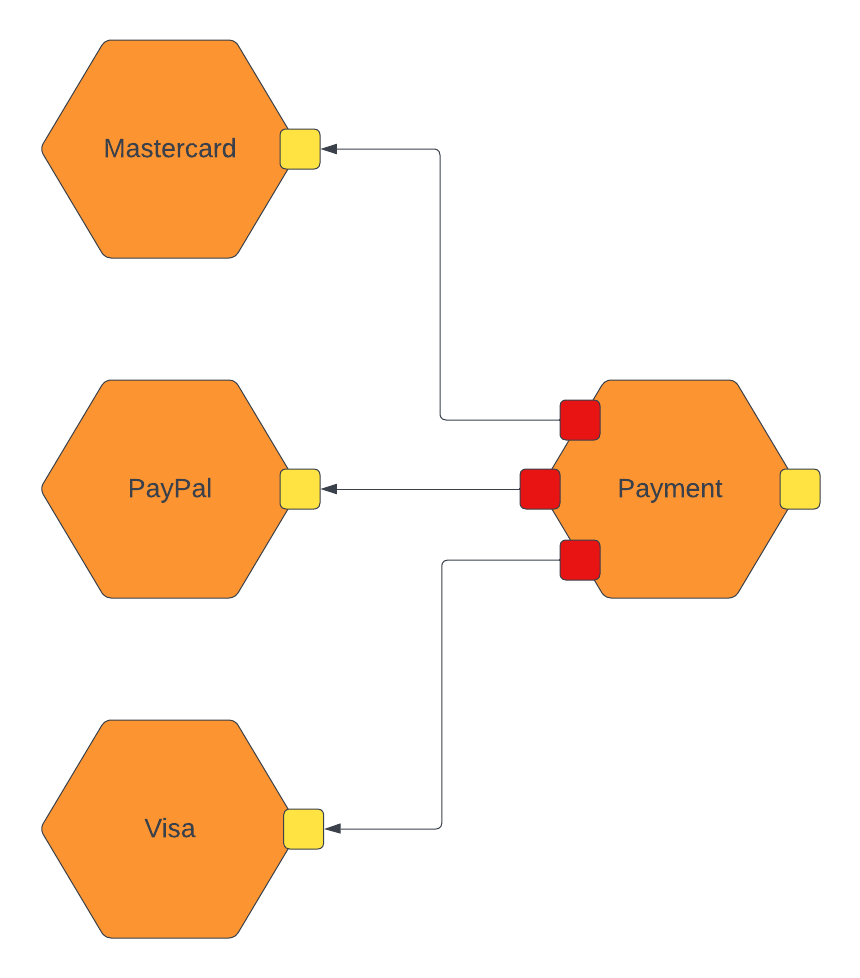
\includegraphics[width=0.5\textwidth]{figures/aggregator_example.png}
    \caption{A group of microservices handling different payment methods. The payment service acts as an aggregator obscuring the underlying services. The orange hexagons depict services, the yellow boxes depict input ports and the red boxes depict output ports.
    Sending a request to the payment service will aggregate the message to the correct payment service depending on the user's chosen payment method. This is done without the client needing to know the correct service's location and protocol.}
    \label{figure:aggregator_example}
\end{figure}
\newdif{Redirection} is a pattern which works similarly to the aggregator, but architecturally is very different.
A service with an input port can specify that a resource name gets redirected to a specific service via an output port.
Listing \ref*{lst:redirector-inputport} displays how an input port can specify resources and map them to an output port.
This means that a client sending a request to the redirector can specify a resource name in the communication media, and the redirector will forward the message to the correct service based on that resource name.
To specify a resource name the client simply needs to specify it in the URL, e.g \texttt{socket://localhost:9000/!/rss} where the \texttt{/!/rss} part is what specifies the resource name.

Redirection can be used to implement several different microservice (API) patterns since it essentially is a proxy.
Generally, a lot of API structures can be implemented using redirectors, because of how a client can specify a specific resource.
\text{API Gateway} is one of the API patterns which can be implemented using redirectors, which are used a lot by heavily visited sites like Netflix.

\begin{jolisting}[][caption={Input port which redirects requests using resource names}, label=lst:redirector-inputport]
inputPort RedirectorPort {
    Location: "socket://localhost:8888"
    Protocol: sodep
    Redirects:
        rss1 => OP1
        rss2 => OP2
}
\end{jolisting}

A simple example of what the redirector could be used for is: imagine that an e-commerce application wants to have one point-of-entry for the system. The application could set up an \textit{API Gateway} which will act as that point of entry. 
When a client wants to get information for a product page, it can specify what it needs in the resource names. This also handles protocol transformation so the client does not need to know the internal service's required protocols.
The example is showcased in figure \ref*{figure:redirector_example}. The client makes requests to the redirector specifying the resource name to fetch the relevant data.
\begin{figure}[h!]
    \center
    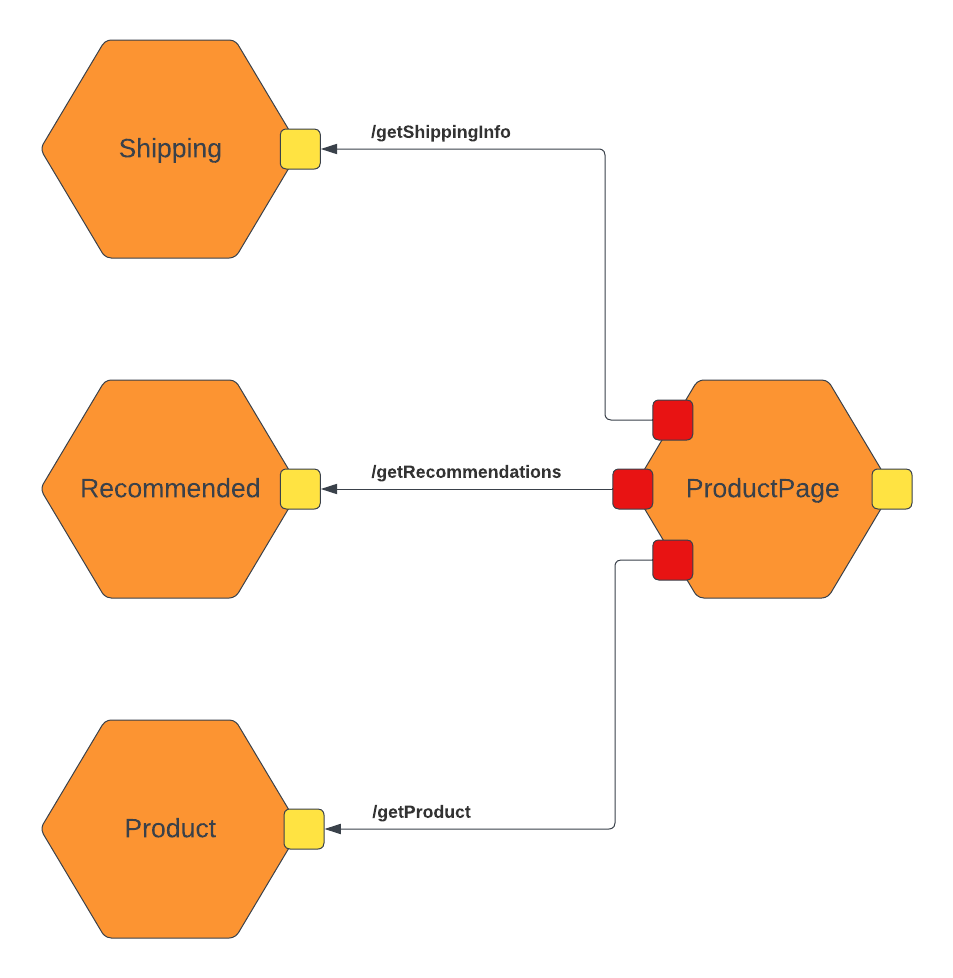
\includegraphics[width=0.5\textwidth]{figures/redirector_example.png}
    \caption{A group of microservices which can be accessed through an API gateway. 
    The client can specify a resource name to specify which service to send the request to.
    The product service fetches information about a product. The recommended service fetches
    the recommended products based on the user and the shipping service fetches shipping information given the user's location.}
    \label{figure:redirector_example}
\end{figure}
\newdif{Couriers}  allow the developer to append functionality to a set of operations. They work well in extension with other communication topologies like aggregators.
The developer defines a courier process by specifying an input port and a set of operations. When that input port receives a request using any of the operations, the courier process executes some code before forwarding
the request along to the main operation implementation.

Couriers can be used to implement any type of middleware functionality. From the book by Olaf Zimmermann et al., many of the quality patterns can be implemented using couriers. This includes
\textit{conditional requests}, \textit{rate limit}, \textit{pricing plan} etc. Besides the quality microservice API patterns, other microservice patterns can be implemented using couriers, namely, \textit{API key} security and authorization.
\newdif{Collections} is another extension of aggregators. Collections are useful when an aggregator input port aggregates services which share the same interface.
They are specified by grouping output ports when defining aggregates.
This together with courier processes can fully, and easily, implement a load balancer for services sharing interfaces because the courier can forward the requests to any of the aggregated services based on some condition.
Since collections are an extension of aggregates, they can have the same use cases, but the collections can group services that share the same interfaces but can have much different underlying business logic.

\section{Docker \& Docker Compose}
Docker is a containerization tool used for deploying applications. It builds an \textit{image} which specifies how the container should build and start when it is created.
Docker handles a single container, and \textit{Docker Compose} is used to handle multi-container applications. Docker Compose will handle the networking between containers, so it is a great tool for testing and deploying applications using a microservice architecture.

Docker Compose is a container orchestration tool, essentially configuring multiple containers and allowing the developer to ensure that the correct files are mounted, the correct ports are exposed and the containers are bound to their specified networks. It also handles multiple instances/replicas
of containers if needed.

\subsection{Jolie in Docker}
\label{label:jolie_in_docker}
To utilize Docker and Docker Compose when developing a microservice architecture in Jolie, creating images can be done using the Jolie base image \texttt{jolielang/jolie}.
Using this image when making a Dockerfile will set up Jolie when building the image, so only the exposed ports, source files and possible runtime arguments should be handled by the developer.

When running a container, the developer needs to specify what container ports to expose, what parameters should be parsed into the Jolie program, and if it needs to connect to other services the developer needs to first create the network and then assign each container to that network.
This is where Docker Compose, or \textit{Kubernetes} which is another container orchestration tool, can become helpful because it will take care of all this if the developer specifies it in the deployment configuration file.

Connecting ports over a Docker network needs some extra work from the developer. Ports which use TCP/IP sockets for communication cannot use "localhost" as seen in the previous examples, they need to use the container name as the host address so Docker can figure out where to send messages inside the network.
This can look something like: \texttt{socket://auth:9999}, where \texttt{auth} is the name of the container.

\section{Current Tools}
Jolie, and other programming languages, do have some tools in order to enhance the developer experience. This section will go through some of the tools
which have been developed for Jolie and then look at some of the counterparts in other languages.
%
\newdif{Joliedoc} generates a documentation page for a single Jolie service. This gives an overview of the API a Jolie service exposes. It shows the input ports and output ports of the service as well as their location and protocol.
This tool is useful when the developer wants a simple and easy-to-follow representation of a single service's API, which include operations, types, port information, and dependencies.
For other programming languages, there are tools like \textit{JSDoc} which look at the comments in the code to generate the API documentation. This requires the developer to write more lines for the same result.
Tools like \textit{Stoplight} and \textit{Swagger} can do the same for all languages, but this requires the developer to set up a markdown or YAML file and specify the whole API in that.
Because of Jolie's way of writing the API as a part of the language, Joliedoc can infer the API from the code without the developer needing to write more lines or comments to achieve this goal.
Jolie does have another tool which generates OpenAPI specifications, which Swagger uses, but this is more to be used in conjunction with these other tools, and is not a standalone tool like Joliedoc is.
% TODO
\newdif{JPM} is a package management tool for Jolie which, similarly to NPM, keeps track of dependencies of a Jolie program.

\subsection{Visualization Tools}
There are a lot of different visualization tools for software architecture which all fall into some categories and all have different use cases and intentions.
The subset of tools which fall under the category of \textit{modelling tools} aims to document a system on different levels of abstraction. This can be on the level of individual components to large-scale businesses with interconnecting components and sectors.
Tools like \textit{IcePanel} and \textit{Aplas} allow the developer of a system to use C4 modelling to create a model of their system, on any level of abstraction.

Another subset of tools is the code-based tools which allow the developer to programmatically or textually create models. This is where tools like \textit{mermaid}, \textit{ELK} and \textit{graphviz} belong.
These tools allow the developer to write structured text or code and then they will render the diagram. Developers do not have to use any specific modelling technique, if they can write it in text or code it will be visualized.

The last relevant category of tools is the diagramming tools. Tools like \textit{draw.io} and \textit{lucidchart} allows the user to diagram everything from E/R, UML and FlowCharts to complex systems.
This is often done in a drag-and-drop fashion.

One thing all these tools have in common is that they need developers to handle the modelling and diagramming. The developers need to have an overview of the system and then model it using any of these tools.
\clearpage